\documentclass[11pt,a4paper]{article}

\usepackage[T1]{fontenc}
\usepackage{mathpazo}
\usepackage[scaled=0.92]{helvet}
\usepackage[margin=2.3cm]{geometry}
\usepackage{microtype}
\usepackage{amsmath}
\emergencystretch=3em
\usepackage{graphicx}
\usepackage{booktabs}
\usepackage{tabularx}
\usepackage{xcolor}
\usepackage{listings}
\usepackage{caption}
\usepackage{float}
\usepackage{placeins}
\usepackage{array}
\renewcommand{\topfraction}{0.85}
\renewcommand{\textfraction}{0.1}
\renewcommand{\floatpagefraction}{0.75}
\renewcommand{\bottomfraction}{0.5}
\usepackage{titlesec}
\usepackage[hidelinks]{hyperref}

\graphicspath{{../figures/}}
\definecolor{accent}{HTML}{000000}
\definecolor{codebg}{HTML}{F5F6F8}
\titleformat{\section}{\Large\bfseries\color{accent}}{\thesection}{0.8em}{}
\titleformat{\subsection}{\large\bfseries}{\thesubsection}{0.8em}{}
\captionsetup{font=small,labelfont=bf}
\setlength{\parskip}{0.45em}
\setlength{\parindent}{0pt}

\lstset{language=Python, basicstyle=\ttfamily\footnotesize, backgroundcolor=\color{codebg},
  frame=single, rulecolor=\color{codebg}, breaklines=true, columns=fullflexible,
  keywordstyle=\color{accent}\bfseries, commentstyle=\color{gray}\itshape,
  stringstyle=\color[HTML]{9C3D10}, showstringspaces=false, xleftmargin=4pt, xrightmargin=4pt}

\newcommand{\pname}[1]{\texttt{#1}}

\title{\bfseries\color{accent} Team Smashcoins at IMC Prosperity 4\\[0.3em]
\large\mdseries\color{black} Strategies, results and a post-mortem}
\author{POON Ka Hang (Jack) \and SIT Chak Hong (Ivan) \and LIN Hao Kun (Jacky) \and CHAN Yui San (Terrence)\\[0.4em]
\small The Hong Kong University of Science and Technology}
\date{April 2026}

\begin{document}
\maketitle

\begin{center}
\fcolorbox{accent}{white}{\begin{minipage}{0.88\textwidth}\vspace{0.4em}
\textbf{Summary.} We finished \textbf{1,032nd of 18,803 teams (top 5.5\%)} in IMC Prosperity 4, a five-round
algorithmic and manual trading competition. Our best standing was \textbf{772nd}, after Round 4, where an
implied-volatility smile strategy with a portfolio delta budget and a long-volatility manual portfolio
earned 82,544 XIRECs. We lost ground in Round 5, where the manual challenge's quadratic fees
outweighed a profitable set of news calls. Re-running statistical checks afterwards also showed that much of
our Round 5 algorithmic evidence could have come from noise alone; Section~\ref{sec:postmortem} sets out
those checks and what we would change.
\vspace{0.4em}\end{minipage}}
\end{center}

\section{Results}

We did not record our profit for Rounds 1 and 2. Those cells are left blank rather than estimated.

\begin{table}[htbp]
\centering\small
\begin{tabular}{@{}c c r r r r@{}}
\toprule
Round & Phase & Algorithmic PnL & Manual PnL & Round PnL & Overall rank after round \\
\midrule
1 & 1 & not recorded & not recorded & not recorded & --- \\
2 & 1 & not recorded & not recorded & not recorded & qualified for Phase 2 \\
3 & 2 & 37,318 (879th) & 75,529 (230th) & 112,847 & 845 \\
4 & 2 & 37,236 (995th) & 45,309 (445th) & 82,544 & \textbf{772} \\
5 & 2 & 39,567 & $-$23,154 & 16,413 & \textbf{1,032 (final)} \\
\bottomrule
\end{tabular}
\caption{Results by round, in XIRECs. Bracketed ranks are within that round only. Phase~2 cumulative PnL after
Round~5 was 211,804.}
\end{table}

\section{The competition and our team}

Prosperity 4 ran as five rounds: Rounds 1--2 lasted 72 hours each and Rounds 3--5 lasted 48 hours each. In every round, teams submitted a Python trading
algorithm that ran against a simulated exchange, plus a separate manual trading decision. Rounds 1--2 were
qualifiers: teams needed a net profit of 200,000 XIRECs (the competition's currency) to continue, after which
the leaderboard reset for Phase 2 (Rounds 3--5).

\begin{table}[htbp]
\centering\footnotesize
\begin{tabularx}{\textwidth}{@{}l >{\raggedright\arraybackslash}X >{\raggedright\arraybackslash}X@{}}
\toprule
Member & Programme (HKUST) & Main contribution \\
\midrule
POON Ka Hang (Jack) & BEng, Computer Science and Mathematics (double major), Business minor &
Rounds 1--2 algorithm; options and volatility-smile strategies in Rounds 3--5; Round 5 product classification \\
SIT Chak Hong (Ivan) & BSc, Biotechnology and Mathematics (double major), Business minor &
Non-options strategies from Round 3 (\pname{HYDROGEL\_PACK}, \pname{VELVETFRUIT\_EXTRACT}); Round 5 products without a clear strategy \\
LIN Hao Kun (Jacky) & BEng, Computer Science, Extended Major in Artificial Intelligence & Manual trading, Rounds 3--5 \\
CHAN Yui San (Terrence) & BSc, Physics & Manual trading, Rounds 3--5 \\
\bottomrule
\end{tabularx}
\caption{Team and division of work.}
\end{table}

\section{Rounds 1--2: market making}

\textbf{Products.} \pname{ASH\_COATED\_OSMIUM}, described as volatile with a possible hidden pattern, and
\pname{INTARIAN\_PEPPER\_ROOT}, described as steady and slow-growing; position limit 80 each. Round~2 kept the
products and added a blind auction: teams could bid, through a \texttt{bid()} function, for 25\% more
order-book volume, with the top half of bids accepted and charged.

\textbf{What we built.} Both rounds used a market maker. The Round~1 file was edited into Round~2 and
not kept, so \texttt{code/round2\_market\_maker.py} is the surviving version. Each tick it:
\begin{itemize}\setlength\itemsep{0.1em}
\item takes a \emph{volume-weighted mid} as the raw fair price, then smooths it with a per-product EMA
(slow for osmium, $\alpha=0.1$; fast for pepper root, $\alpha=0.4$);
\item skews fair value against the current position, so a long book quotes lower and sheds inventory;
\item widens the quoted spread with a 10-tick rolling volatility;
\item takes any quote at least half a tick through skewed fair value, then penny-jumps the best bid and ask
without quoting inside its target edge.
\end{itemize}

\textbf{What we missed.} The code capped positions at \textbf{20} when the exchange allowed \textbf{80}, using a
quarter of the available capacity. It also had no \texttt{bid()} function, which the rules treat as a bid of
zero, so we did not compete for the extra volume. We do not have the manual-round decisions for Rounds 1--2
(an opening auction in Round 1 and a budget allocation across research, scale and speed in Round 2).

\section{Round 3: fair-value models and a first volatility smile}

\textbf{Products.} \pname{HYDROGEL\_PACK}, \pname{VELVETFRUIT\_EXTRACT} and ten call vouchers on the extract,
\pname{VEV\_4000} to \pname{VEV\_6500}.

\subsection{Non-options strategy (Ivan)}
Ivan compared several fair-value estimators on \pname{HYDROGEL\_PACK} (a weighted average price (WAP) based
on order-flow imbalance, a Kalman filter, an EWMA and a Bayesian update from trade prints; Figure~\ref{fig:fv}
compares the first three) alongside order-flow maps and a mean-reversion rule. The submitted
algorithm (\texttt{code/round3\_bayesian\_mean\_reversion.py}) updates fair value with a precision-weighted
Bayesian step for every market trade, where larger trades carry more weight. It enters when price deviates from
fair value by more than a threshold that scales with recent volatility, observes a cooldown between entries, and
exits when price crosses back through fair value.

For a trade at price $p$ and size $q$, the observation noise is $\sigma_{\text{obs}}=2/\sqrt{|q|}$, and the
fair value $\mu$ and its uncertainty $\sigma$ update as
\[
\mu \leftarrow \frac{\mu/\sigma^2 + p/\sigma_{\text{obs}}^2}{1/\sigma^2 + 1/\sigma_{\text{obs}}^2},
\qquad
\sigma^2 \leftarrow \frac{1}{1/\sigma^2 + 1/\sigma_{\text{obs}}^2}.
\]
The entry threshold is $\theta=\theta_0+z\,\sigma\,v$, where $v$ is the coefficient of variation of the last
20 mid prices. For \pname{HYDROGEL\_PACK}, $\theta_0=0.5\%$, $z=2.5$ and the cooldown is 5,000 timestamps;
each entry uses 20\% of the 200-lot limit. One limitation: with no process-noise term, $\sigma$ only ever
shrinks, so the longer the round runs, the less the fair value responds to new trades. A Kalman filter, one of
the alternatives Ivan tested, adds that term.

\begin{figure}[htbp]
\centering
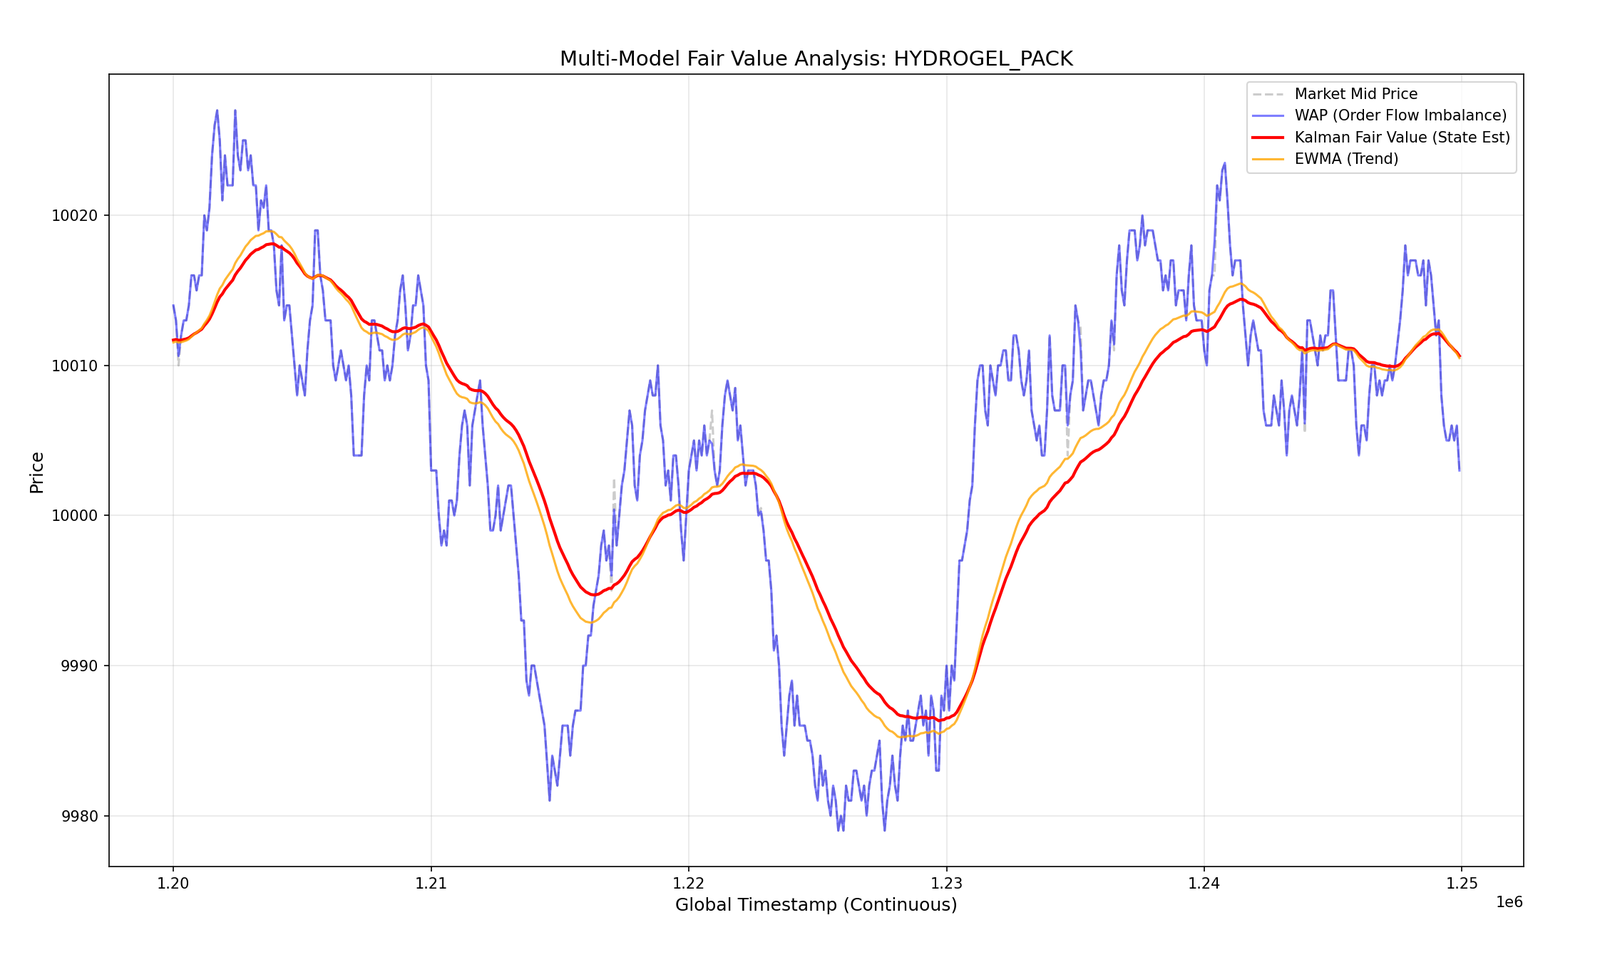
\includegraphics[width=\textwidth]{r3_hydrogel_fair_value_models.png}
\caption{WAP, Kalman filter and EWMA fair-value estimates against the \pname{HYDROGEL\_PACK} mid price.}
\label{fig:fv}
\end{figure}

\FloatBarrier
\subsection{Options research (Jack)}
For each voucher, Jack backed out implied volatility with Black--Scholes and plotted it against log-moneyness
scaled by time to expiry, $m=\ln(S/K)/\sqrt{T}$. This collapsed the strikes onto a single parabola
(Figure~\ref{fig:smile3}); in this convention the first fit was $\sigma(m)=0.1768m^2+0.006588m+0.1946$. Across 300,000 observations,
market IV sat on average 0.090 below the curve, with a standard deviation of 0.206. A screen on liquidity, vega,
stability of the residual and book depth ranked strikes 5000--5400 as the best candidates.

The trading version was not ready in time. The submitted file only mirrored the underlying's signal on four
strikes, which added directional exposure rather than trading volatility. We count this round's options work as
unsuccessful; it became the basis for Round~4.

\begin{figure}[htbp]
\centering
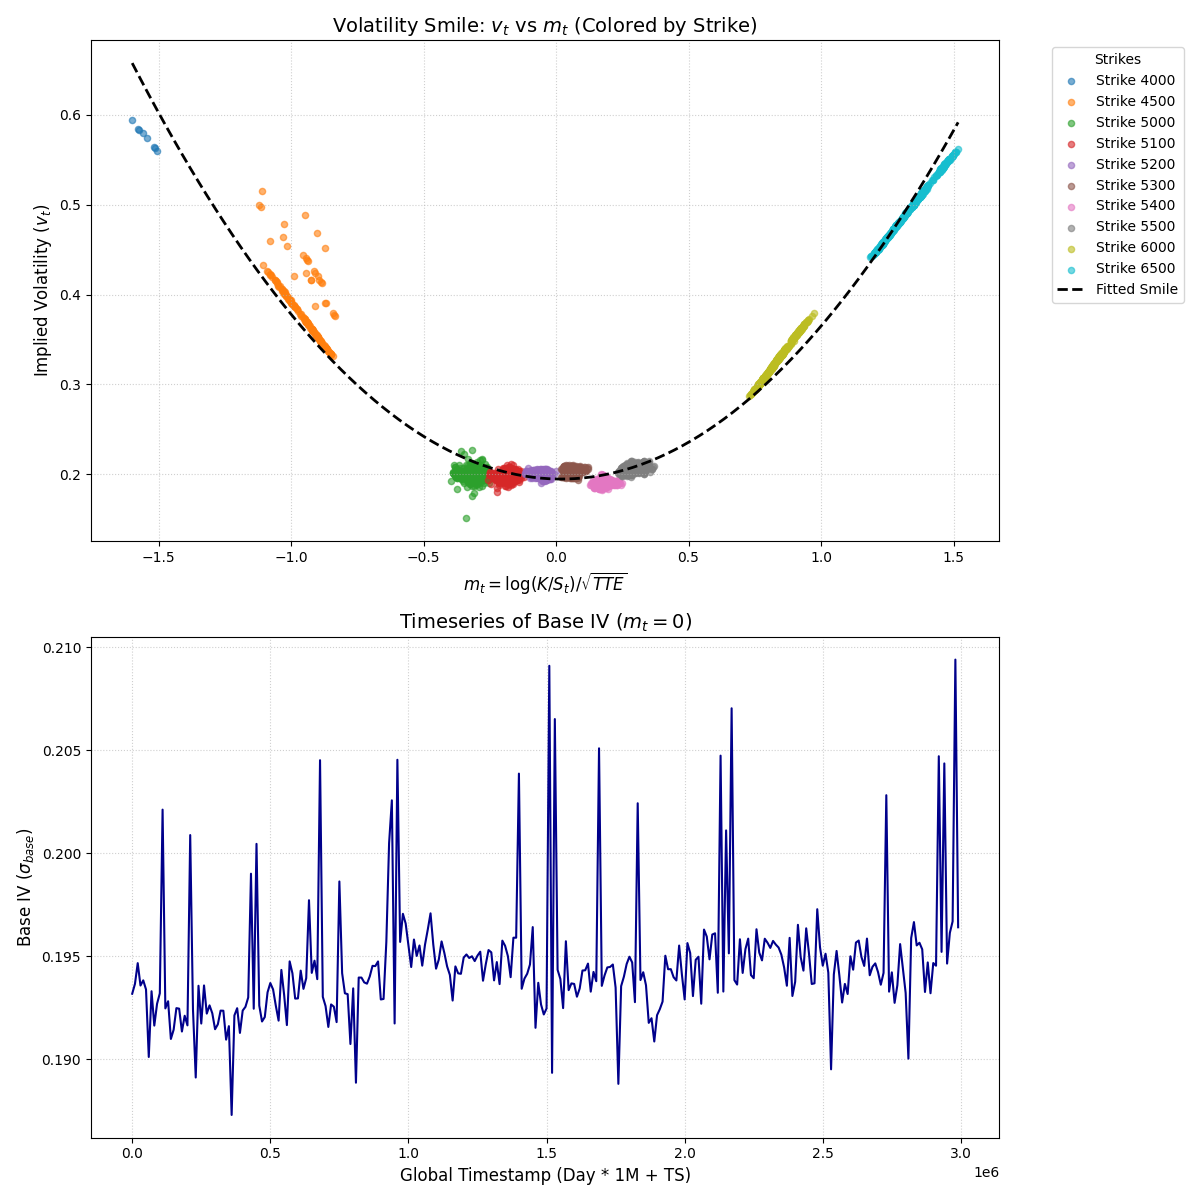
\includegraphics[width=0.62\textwidth]{r3_vev_volatility_smile.png}
\caption{Implied volatility against moneyness, coloured by strike, with the fitted parabola (top), and the
fitted base IV over the round (bottom). This chart plots $\ln(K/S)/\sqrt{T}$, the mirror image of $m$, so the
curve's linear term appears here with the opposite sign.}
\label{fig:smile3}
\end{figure}

\begin{figure}[htbp]
\centering
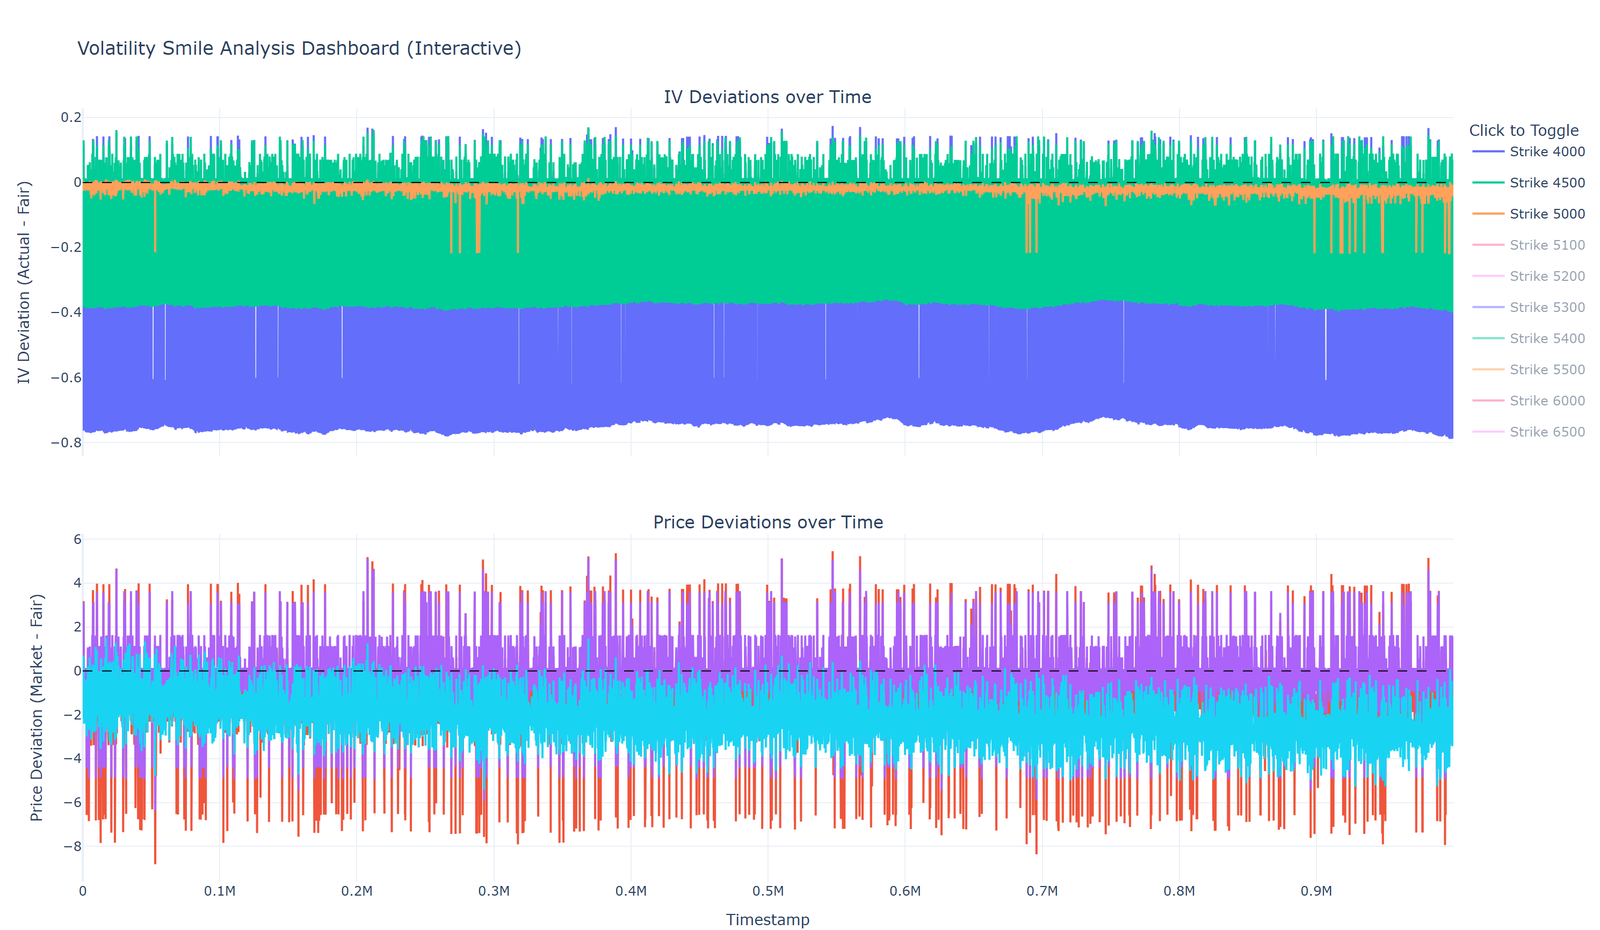
\includegraphics[width=\textwidth]{r3_vev_iv_deviation.png}
\caption{Deviation of market IV (top) and market price (bottom) from the fitted curve over time, by strike.}
\label{fig:ivdev}
\end{figure}

\FloatBarrier
\subsection{Manual trading (Jacky and Terrence)}
For the first bid, they assumed counterparties' reserve prices were uniform between 670 and 920 and that bought
inventory could be resold at 920. Expected profit per counterparty is then
$P(\text{win})\times(920-b)$, which peaks at bids of 790--795 (about 63.7). They chose 795 for the higher chance
of trading. The second bid's payoff depended on other teams, so they estimated where the field's average bid
would land and whether the public would bid above or below it.

\textbf{Result:} algorithmic +37,318 (879th in the round) and manual +75,529 (230th), a round total of
112,847; overall rank 845. This was the manual team's best round.

\FloatBarrier
\section{Round 4: the implied-volatility smile scalper}

\subsection{Options algorithm (Jack)}
Jack's options component (\texttt{code/round4\_iv\_smile\_scalper.py}) turned the Round~3 research into a
strategy; Ivan ran the non-options products. Each tick, the algorithm:
\begin{enumerate}\setlength\itemsep{0.1em}
\item computes \textbf{fair IV} per strike from the refitted smile, $\sigma(m)=0.1762m^2+0.007389m+0.1946$,
almost the same curve as the Round~3 fit, so the smile was stable across rounds;
\item inverts the market mid to \textbf{market IV} by bisection, in pure Python using only the standard
\texttt{math} library (SciPy was not supported on the exchange);
\item trades the \textbf{IV residual with hysteresis}: enter beyond $\pm1.5$ volatility points, hold in between,
exit inside $\pm0.5$;
\item \textbf{sizes by conviction} (25 lots at the entry threshold, up to 150) and only walks the order book up
to the model price;
\item enforces a \textbf{portfolio delta budget} and hedges the forward-looking delta with the underlying.
\end{enumerate}
\begin{figure}[htbp]
\centering
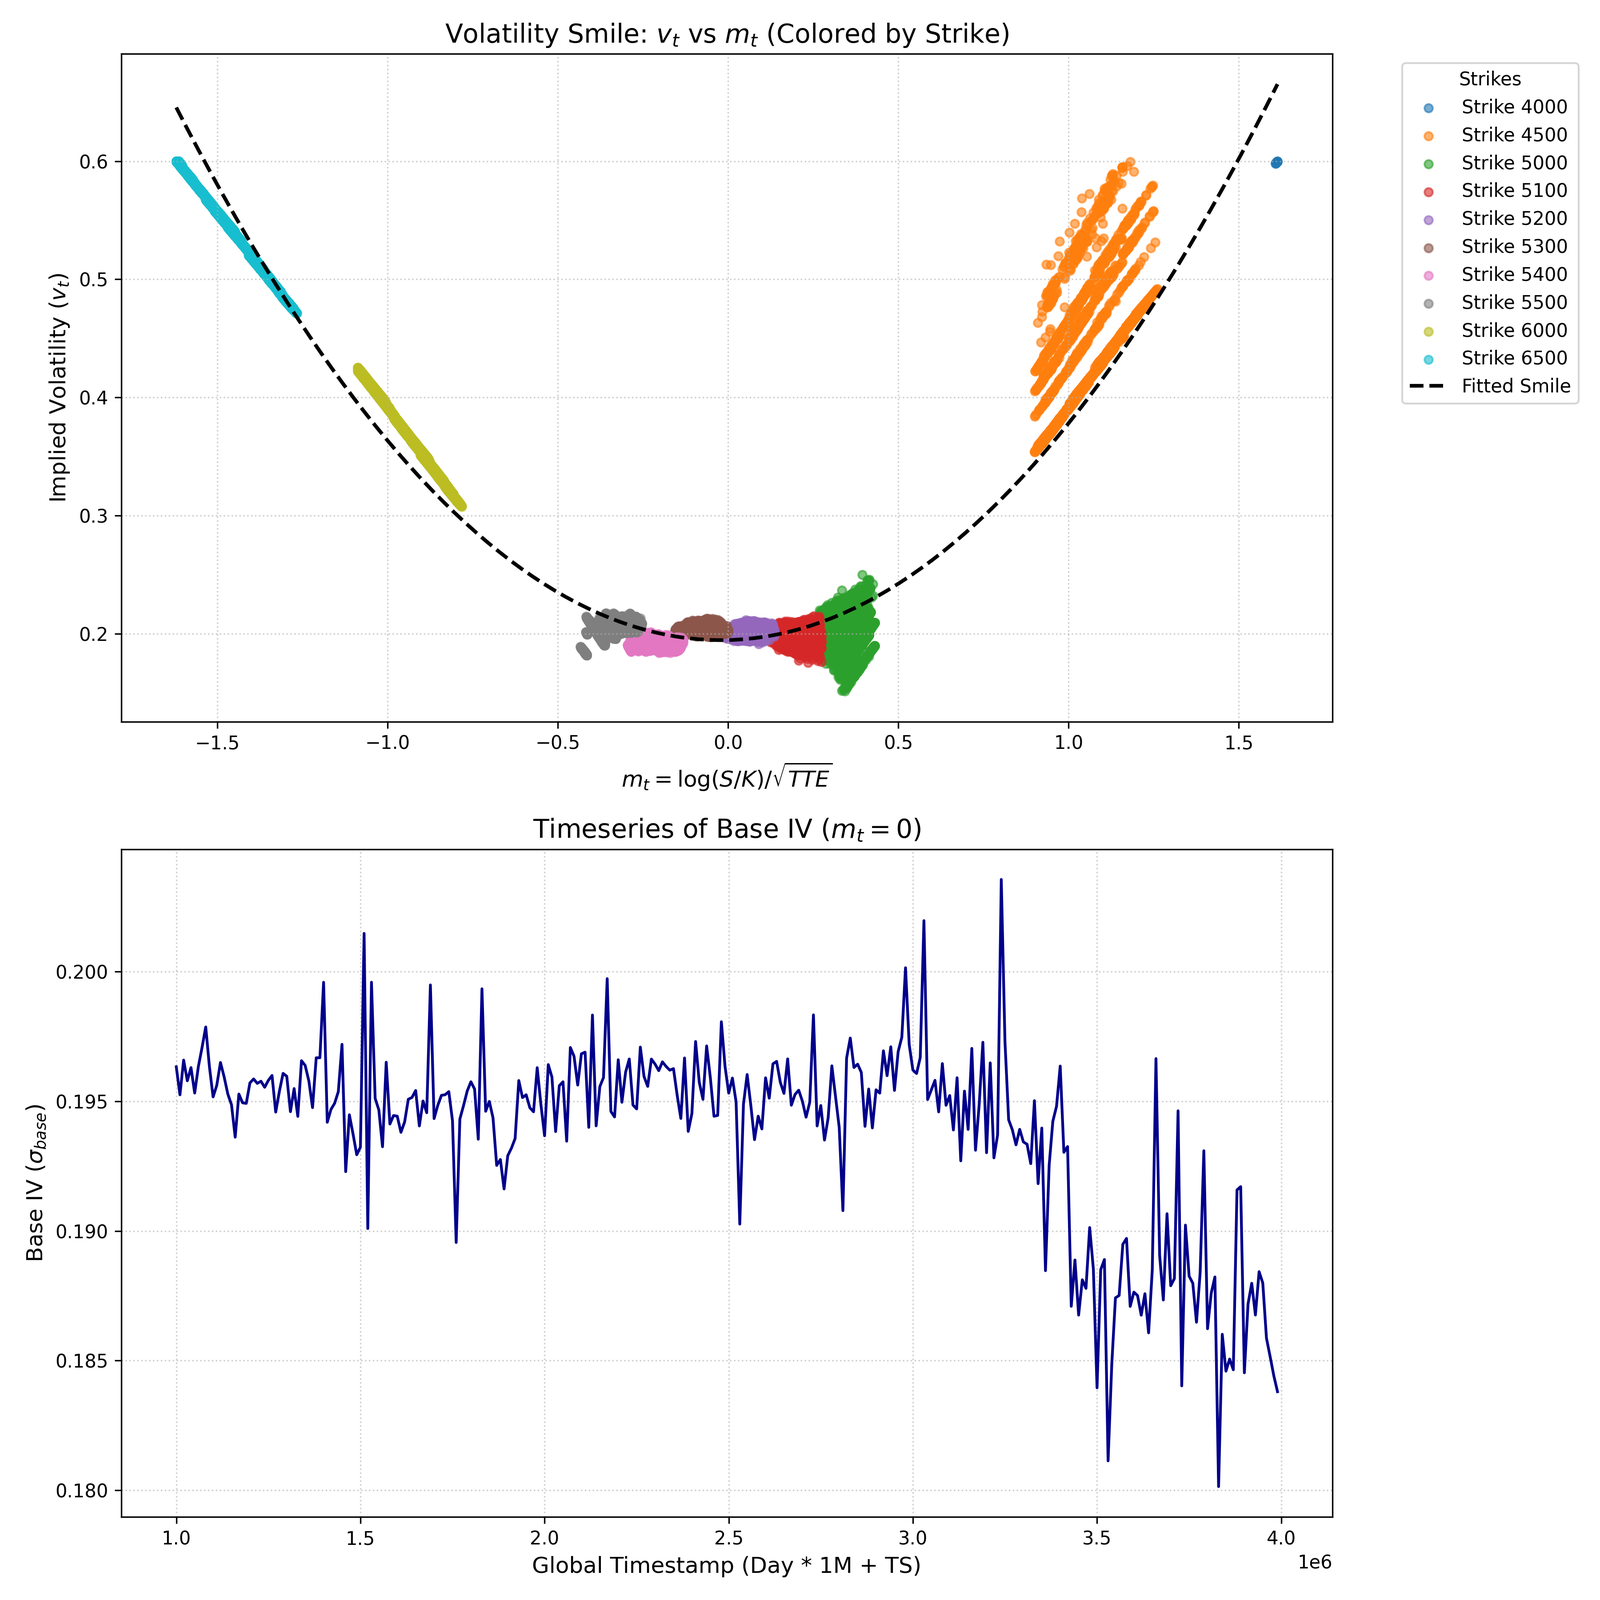
\includegraphics[width=0.5\textwidth]{r4_vev_volatility_smile_refit.png}
\caption{The refitted smile used in the Round 4 submission.}
\end{figure}

In symbols, with residual $\Delta\sigma=\sigma_{\text{mkt}}-\sigma_{\text{fair}}$, the target position per
strike is
\[
n^\ast=-\operatorname{sign}(\Delta\sigma)\,\min\!\Big(\operatorname{round}\big(25\,|\Delta\sigma|/0.015\big),\,150\Big)
\quad\text{when } |\Delta\sigma|>0.015,
\]
and the hedge in the underlying targets $-\sum_k n_k\,\delta_k$, clipped to $\pm200$, where $\delta_k$ is the
Black--Scholes delta at fair IV. Time to expiry is measured in trading days, with $T$ in years on a 252-day
basis.

Deep in-the-money strikes (\pname{VEV\_4000}, \pname{VEV\_4500}) were excluded: with vega close to zero, their
implied volatility was numerically unstable.

The delta budget fixed a capacity problem. Eight strikes at a 200-lot cap and an average delta of 0.5 could
build 800 units of delta, against only 200 units of hedge capacity in the underlying. Capping the book at 175
kept every position hedgeable:

\noindent\begin{minipage}{\linewidth}
\begin{lstlisting}
new_rd = running_delta + want * delta
if new_rd > self.MAX_PORTFOLIO_DELTA:          # 175, below the 200 hedge limit
    want = max(0, int((self.MAX_PORTFOLIO_DELTA - running_delta) / max(delta, 1e-4)))
elif new_rd < -self.MAX_PORTFOLIO_DELTA:
    want = min(0, int((-self.MAX_PORTFOLIO_DELTA - running_delta) / max(abs(delta), 1e-4)))
\end{lstlisting}
\end{minipage}



\FloatBarrier
\subsection{Manual trading (Jacky and Terrence)}
The manual challenge offered calls and puts on a new underlying, \pname{AETHER\_CRYSTAL} (trading at about 50),
with two- and three-week expiries, plus three exotic contracts: a chooser option that becomes a call or a put
after two weeks, a binary put paying 10 if the price finishes below 40, and a put struck at 45 that is knocked
out if the price ever trades below 35. Positions were held to expiry, so the task was pricing: find contracts
quoted away from their expected payoff.

Jacky and Terrence rebuilt the price model the rules described: zero-drift geometric Brownian motion with
251\% annual volatility, four steps per trading day and a 252-day year. The exchange scored each portfolio on its
average profit across 100 simulated paths. Their engine
(\texttt{code/round4\_manual\_options\_engine.py}) priced every contract over 50,000 simulated paths, applying
each exotic's path-dependent rule, and compared the result with the quoted bid and ask (Table~\ref{tab:r4fair}).
The engine, however, used 14 and 21 days for the two- and three-week expiries, while the rules defined them as 10
and 15 trading days.

\begin{table}[htbp]
\centering\small
\begin{tabular}{@{}l l r r r r@{}}
\toprule
 & & & & \multicolumn{2}{c}{Model value} \\
\cmidrule(l){5-6}
Contract & Type & Bid & Ask & Team engine & Official expiries \\
\midrule
\pname{AC\_50\_C} & call, 50, 3 weeks & 12.00 & 12.05 & 14.23 & 12.03 \\
\pname{AC\_50\_P} & put, 50, 3 weeks & 12.00 & 12.05 & 14.06 & 11.95 \\
\pname{AC\_60\_C} & call, 60, 3 weeks & 8.80 & 8.85 & 11.10 & 8.78 \\
\pname{AC\_45\_P} & put, 45, 3 weeks & 9.05 & 9.10 & 10.99 & 9.01 \\
\pname{AC\_40\_P} & put, 40, 3 weeks & 6.50 & 6.55 & 8.22 & 6.43 \\
\pname{AC\_35\_P} & put, 35, 3 weeks & 4.33 & 4.35 & 5.80 & 4.27 \\
\pname{AC\_50\_C\_2} & call, 50, 2 weeks & 9.70 & 9.75 & 11.63 & 9.92 \\
\pname{AC\_50\_P\_2} & put, 50, 2 weeks & 9.70 & 9.75 & 11.53 & 9.82 \\
\pname{AC\_50\_CO} & chooser, 50 & 22.20 & 22.30 & 25.76 & 21.82 \\
\pname{AC\_40\_BP} & binary put, 40, pays 10 & 5.00 & 5.10 & 5.21 & 4.75 \\
\pname{AC\_45\_KO} & knock-out put, 45, barrier 35 & 0.150 & 0.175 & 0.13 & 0.21 \\
\bottomrule
\end{tabular}
\caption{Round 4 manual quotes against model values from the team's engine (14 and 21 days) and from the same
engine with the official expiries (10 and 15 trading days); 50,000 simulated paths each.}
\label{tab:r4fair}
\end{table}

They decided not to sell options outright, reasoning that a short option has limited profit and unlimited loss,
and built a long-volatility portfolio: two three-week 50 calls and one 50 put (a straddle tilted towards a rise),
one 60 call sold against the calls to recover some premium, the 40 and 35 puts as layered downside protection,
and a two-week 50 call. With the engine's settings, the portfolio's simulated expected profit was +27,382,
but its median was only +480: most paths lost a little and a minority won a lot (Figure~\ref{fig:r4manual}).

\begin{figure}[htbp]
\centering
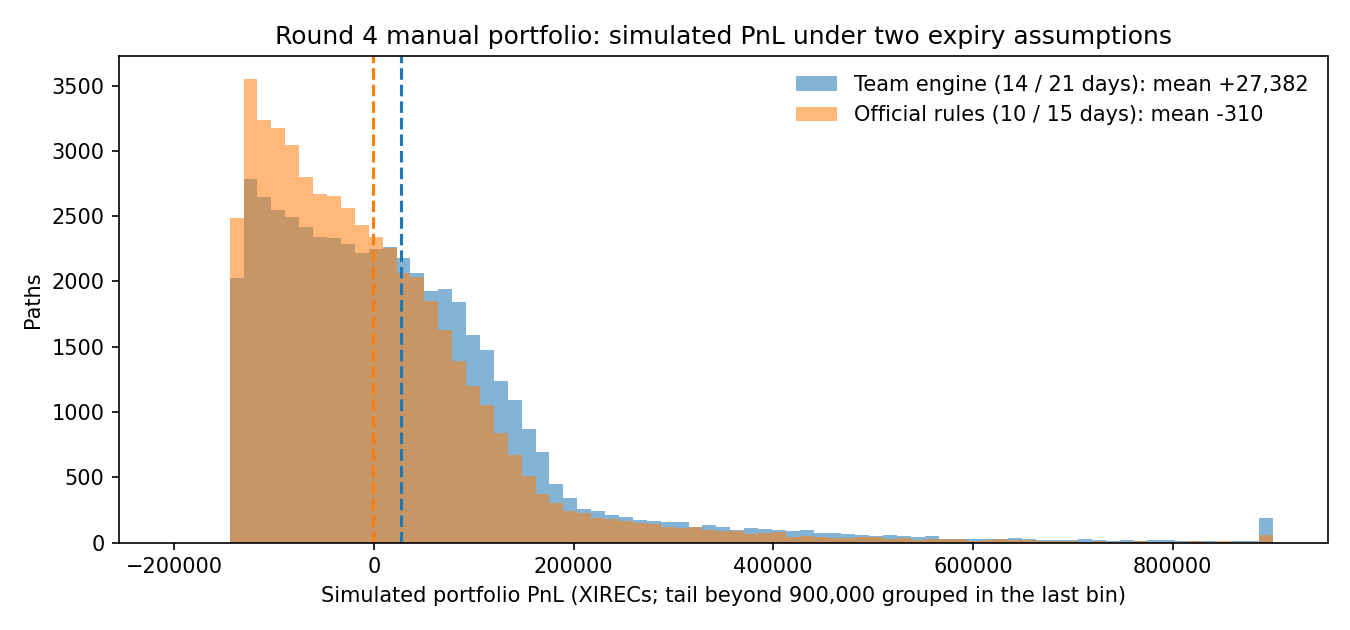
\includegraphics[width=0.9\textwidth]{r4_manual_pnl_engine_vs_official.png}
\caption{Simulated profit of the Round 4 manual portfolio over 50,000 paths, with the engine's expiries and with
the official ones; dashed lines mark the means.}
\label{fig:r4manual}
\end{figure}

The expiry mismatch changes the conclusion. The extra time inflated every vanilla model value by 16--34\%,
which is why every vanilla option looked cheap to the engine. With the official expiries, every vanilla model
value lies within about 2\% of its quote: the vanillas were fairly priced. The genuine mispricings were in the
exotics. The binary put was quoted about 6\% above its value (5.05 against 4.75), and the knock-out put below
its value (0.16 against 0.21), though at a very small size. Under the official settings, the portfolio's expected
profit is close to zero, so its +45,309 came from the 100 price paths the exchange simulated rather than from a
pricing edge.

\begin{figure}[htbp]
\centering

\includegraphics[width=0.72\textwidth]{r4_official_results.png}
\caption{Official Round 4 results screen.}
\end{figure}

\textbf{Result:} algorithmic +37,236 (995th in the round), manual +45,309 (445th), round total 82,544. Our overall
rank improved from 845 to \textbf{772}, the best of the competition. The manual side contributed more than the
algorithm this round.


\FloatBarrier
\section{Round 5: fifty new products}

\subsection{Algorithm (Jack and Ivan)}
Round~5 introduced 50 products in ten families (for example Pebbles, Microchips, UV Visors and Robots), each
with a position limit of only 10. Jack and Ivan split the work by product type. We screened all 50 products
on Hurst exponent, lag-1 autocorrelation (AC1), spread, drift, skew and kurtosis; assigned the clear cases to a
strategy; and left the unclear products to Ivan.

\begin{figure}[htbp]
\centering
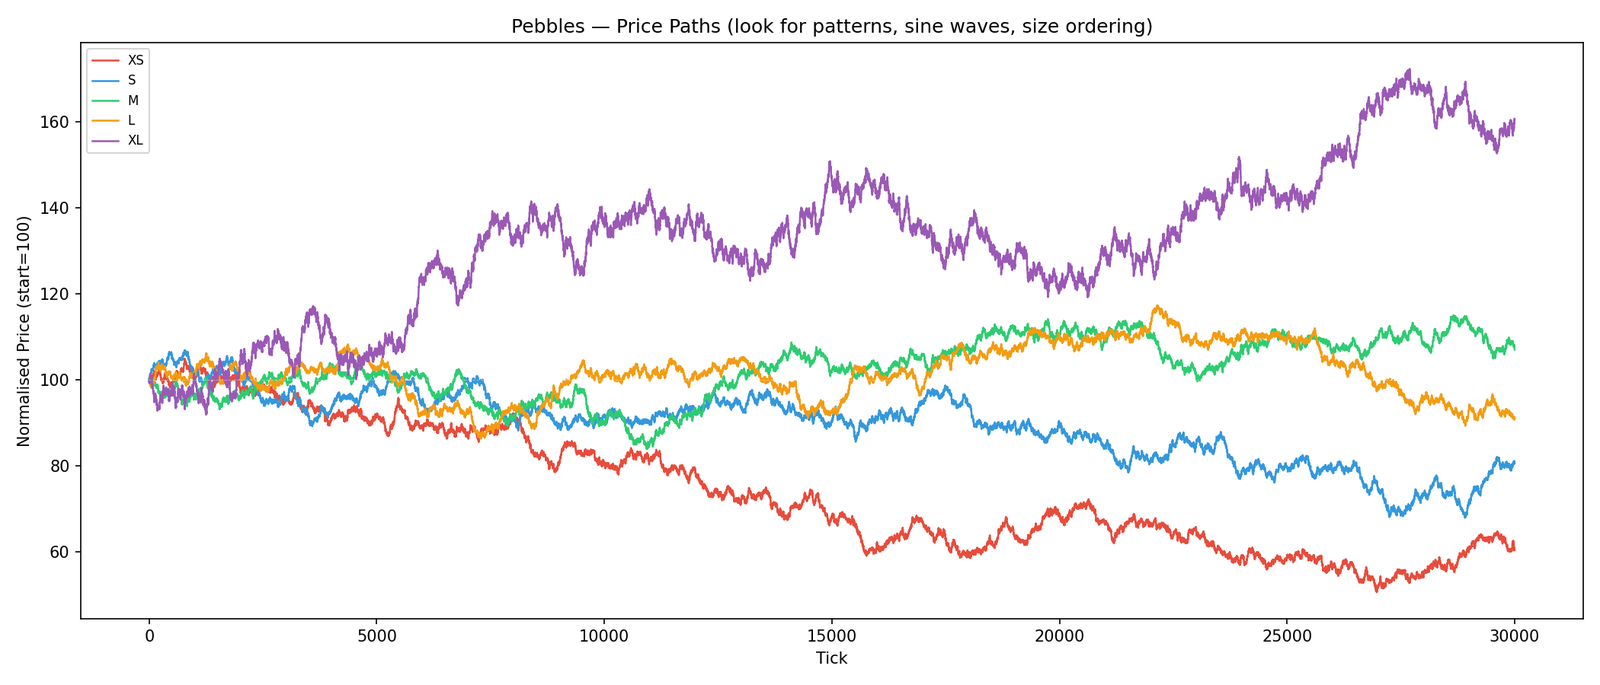
\includegraphics[width=\textwidth]{r5_pebbles_price_paths.png}\\[0.6em]
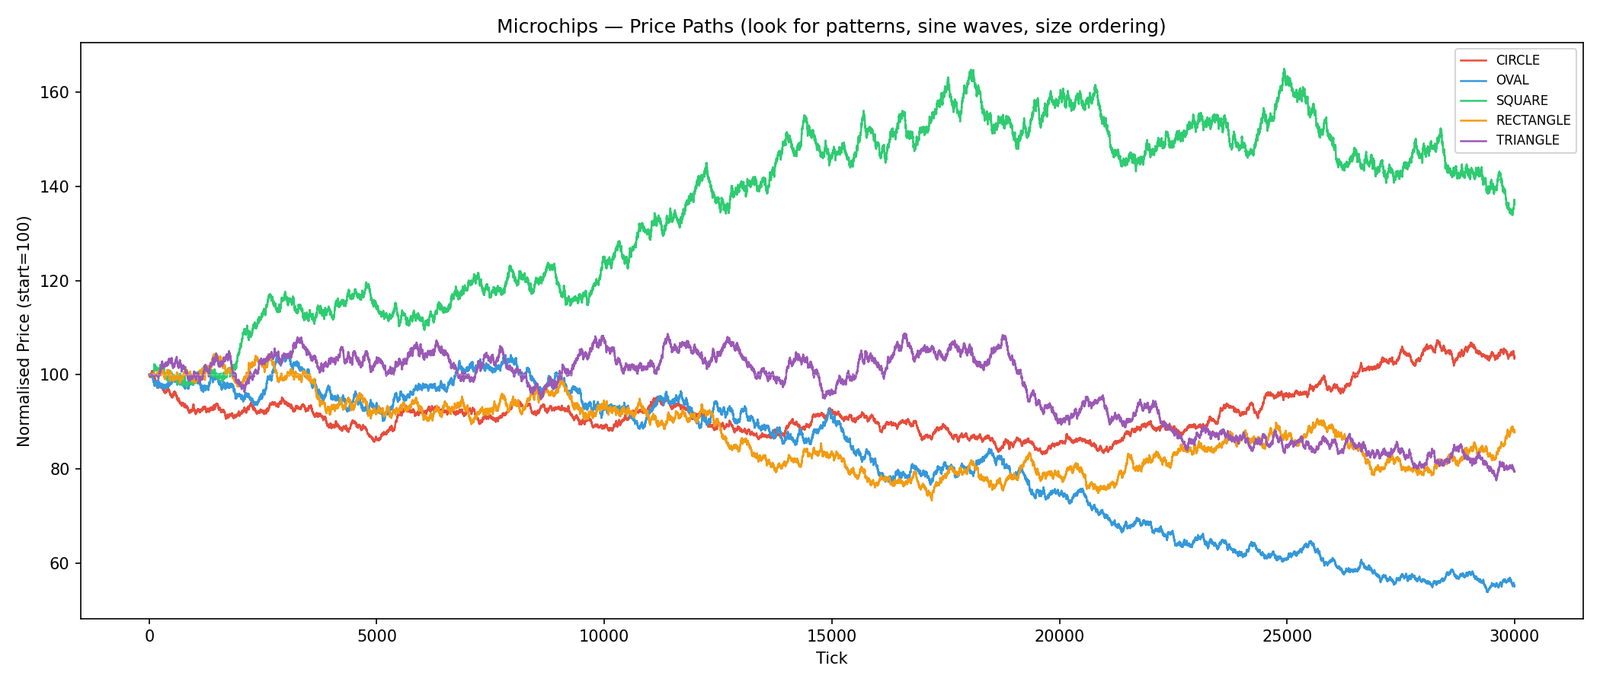
\includegraphics[width=\textwidth]{r5_microchips_price_paths.png}
\caption{Normalised historical price paths for the Pebbles (top) and Microchips (bottom) families.}
\end{figure}

\begin{itemize}\setlength\itemsep{0.1em}
\item \textbf{Market making} (\texttt{code/round5\_market\_maker.py}) on products with negative AC1, such as
\pname{ROBOT\_DISHES} (AC1 $=-0.22$). Its ``wall mid'' fair price and take-then-make structure were adapted
from open-source Prosperity~3 code published by team Frankfurt Hedgehogs. Fair value is the midpoint of the
outermost bid and ask, which is steadier than the touch when the top of book is thin. It first takes any quote at
least one tick through fair value, then quotes one tick inside the outer walls, skewed by up to two ticks against
inventory, and penny-jumps resting orders only if they are larger than a minimum size, to avoid 1-lot bait
quotes.
\item \textbf{Directional holds} (\texttt{code/round5\_directional\_hold.py}): maximum long or short positions
in six products with strong linear trends in the historical data. Attribute patterns motivated the choice:
pebble drift rose with size ($r=0.92$ against mass) and microchip drift with perimeter ($r=0.91$). The book
was short \pname{PEBBLES\_XS}, \pname{MICROCHIP\_OVAL} and \pname{UV\_VISOR\_AMBER}, and long
\pname{PEBBLES\_XL}, \pname{MICROCHIP\_SQUARE} and \pname{UV\_VISOR\_MAGENTA}, each at the 10-lot limit.
\item \textbf{Pairs trading} within families whose price spreads passed an Engle--Granger cointegration test.
\item \textbf{Per-product parameter search}: for each market-making product, the best of eight parameter sets
on the historical data.
\end{itemize}



\FloatBarrier
\subsection{Manual trading (Jacky and Terrence)}
The manual challenge was a one-day news trade on a second exchange, Ignith. Teams could buy or sell any of nine
goods with a budget of 1,000,000 and hold until the next day. Each position paid a fee of
$(v/100)^2\times1{,}000{,}000$, where $v$ is the percentage of the budget allocated to it; unused budget simply
expired.

Jacky and Terrence read the nine stories in the Ashflow Alpha news feed and, for each good, wrote down the
expected direction, the argument for it and the strongest argument against it, then ranked their conviction.
They spread the whole budget across seven goods (Table~\ref{tab:r5manual}).

\begin{table}[htbp]
\centering\small
\begin{tabular}{@{}l l r r r@{}}
\toprule
Good & Side & Allocation & Fee & P\&L after fees \\
\midrule
Lava cake & Sell & 23\% & 52,900 & +92,813 \\
Magma ink & Buy & 15\% & 22,500 & $-$19,159 \\
Thermalite core & Buy & 5\% & 2,500 & +8,580 \\
Ashes of the Phoenix & Sell & 17\% & 28,900 & $-$22,943 \\
Scoria paste & Buy & 15\% & 22,500 & $-$20,501 \\
Obsidian cutlery & Sell & 15\% & 22,500 & $-$37,374 \\
Volcanic incense & Buy & 10\% & 10,000 & $-$24,571 \\
\midrule
Total & & 100\% & 161,800 & $-$23,154 \\
\bottomrule
\end{tabular}
\caption{Round 5 manual positions, from the official manual results screen.}
\label{tab:r5manual}
\end{table}

Five of the seven directional calls were right, and before fees the positions made about +138,600. The fees came
to 161,800. Under the fee rule, allocating $v\%$ of the budget $B$ to a good that moves by a fraction $\mu$ earns
$B\,(\mu v/100-(v/100)^2)$, which is positive only if $\mu>v/100$: a $v\%$ allocation needs a price move of
more than $v\%$ just to break even. Lava cake (23\%) moved about 63\% and cleared that bar easily, and
Thermalite core (5\%) moved about 22\%. Ashes of the Phoenix (17\%), Magma ink and Scoria paste (15\% each)
were right on direction but moved only 1--4\%, far short of their break-even. Maximising the same expression
gives $v^\ast=50\mu$: a good expected to move 10\% deserved only 5\% of the budget, and nothing required
spending all of it.

The team's trading journal records two further lessons. Obsidian cutlery was switched from buy to sell in the
final minutes after a split decision, and its size was increased; the market treated the factory accident as a
supply shortage, which pushes the price up, rather than a safety scare. For Magma ink, the pen's built-in ink
reservoir may have reduced short-term demand for ink rather than raised it.

\textbf{Result:} algorithmic +39,567 and manual $-$23,154, a round total of 16,413. We finished \textbf{1,032nd},
down from 772nd. The algorithm earned slightly more than in Rounds 3 and 4, while the manual trade lost money. We
did not log live profit by product, so we cannot say which algorithmic components contributed.

\FloatBarrier
\section{Post-mortem: what pure noise looks like}
\label{sec:postmortem}

After the competition we asked how much of our Round~5 evidence a market with \emph{no signal at all} would
produce. Each check simulates random walks; the code is in the companion notebook, with fixed seeds.

\begin{figure}[htbp]
\centering
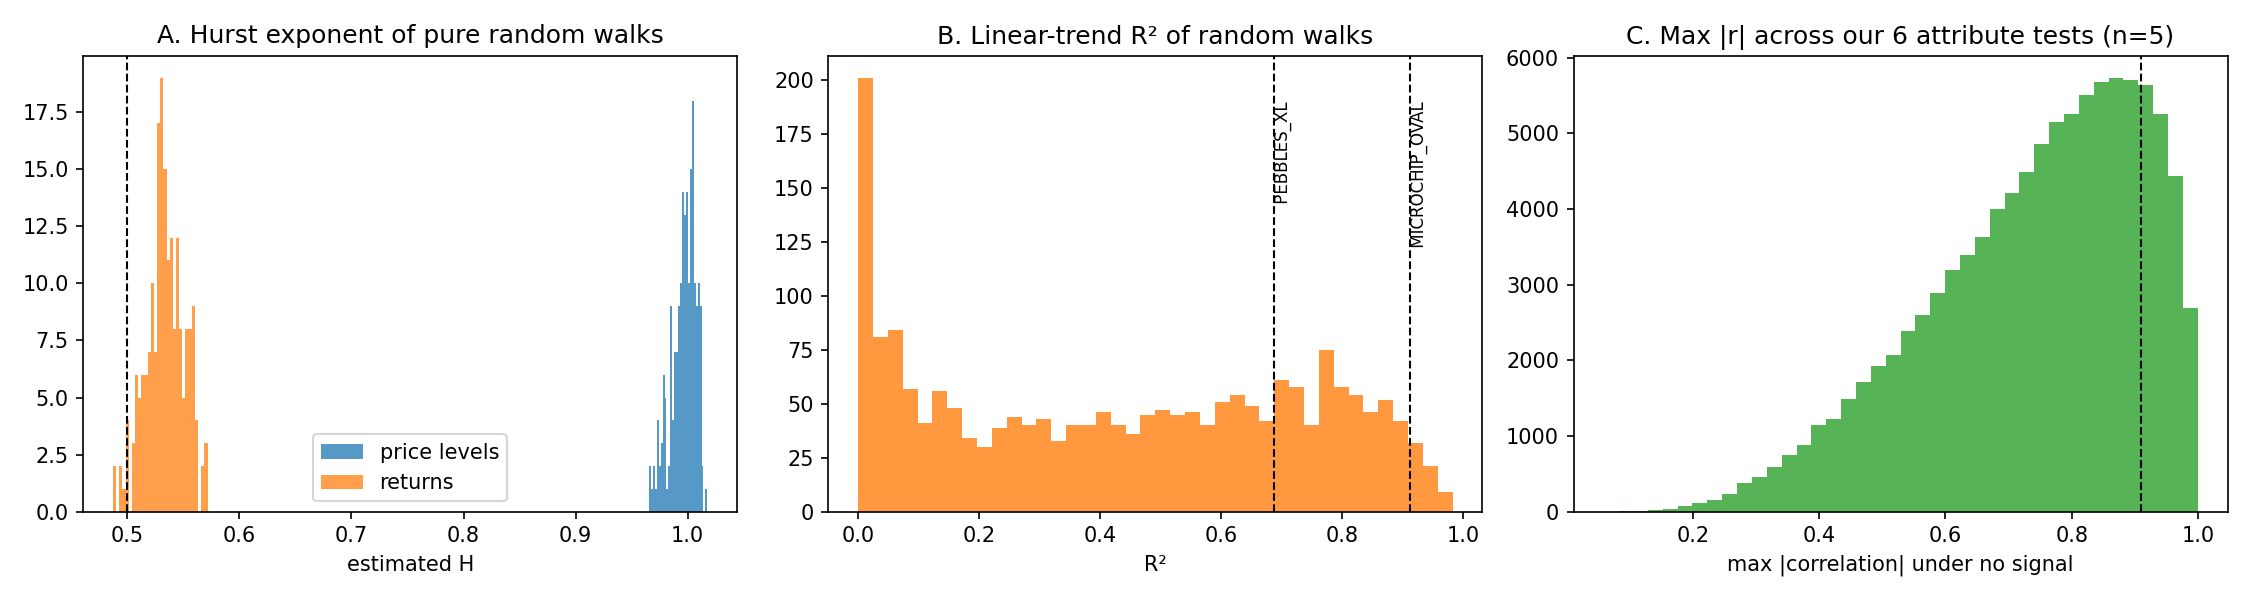
\includegraphics[width=\textwidth]{post_mortem_null_tests.png}
\caption{Null simulations. (A) Hurst exponent of random walks on price levels vs.\ returns. (B) Linear-trend
$R^2$ of 30,000-tick random walks, with two of our directional picks marked. (C) Largest $|r|$ across our six
attribute tests when drifts are pure noise; the dashed line is $r=0.91$.}
\end{figure}

\begin{enumerate}
\item \textbf{The Hurst exponent was measured on the wrong series.} On price \emph{levels}, a random walk gives
$H\approx1.0$ (median 0.998 in 200 simulations), compared with about 0.53 on returns. Our screen used levels,
which is why 46 of 50 products were labelled ``trending''. The label carried no information.
\item \textbf{Strong-looking trends are common in noise.} Fitting a straight line to a 30,000-tick random walk
gives a median $R^2$ of 0.44; 26\% of walks exceed 0.7 and 3.6\% exceed 0.9. Among 50 noise products we should
expect about 13 above 0.7. Our directional picks had $R^2$ between 0.69 and 0.91.
\item \textbf{Five data points cannot confirm a pattern.} With five products per family, a correlation of 0.91
occurs 3.2\% of the time for one test. Trying six attributes, as we did, raises that to 17\%. The size and
perimeter patterns were reasonable hypotheses, not discoveries.
\item \textbf{Choosing the best of eight parameter sets flatters the backtest.} For a strategy with zero edge,
the best of eight backtests is expected to show +1.0 to +1.4 standard deviations of profit, depending on how
correlated the sets are. Our per-product backtest figures were optimistic by construction.
\end{enumerate}

None of this proves our Round~5 strategies were wrong. It shows that our evidence could not distinguish them
from noise, and that is the first thing we would test next time.

\subsection*{What we would do differently}
\begin{enumerate}\setlength\itemsep{0.1em}
\item \textbf{Hold out a day.} Fit on two days of history and require the signal to survive on the third before
trading it.
\item \textbf{Test returns, not prices}, and require trends to persist out of sample rather than relying on $R^2$.
\item \textbf{Log live profit by product and component}, so a weak round can be diagnosed.
\item \textbf{Use every lever the round offers}: the full position limit and every bidding mechanism.
\item \textbf{Size to the fee.} In the Round~5 manual challenge, a $v\%$ allocation needed more than a $v\%$ move
to break even; we spent the full budget and paid more in fees than the positions earned.
\item \textbf{Check units against the rules.} In the Round~4 manual challenge, expiries counted in calendar
days instead of trading days made every vanilla option look 16--34\% cheap.
\item \textbf{Keep what worked}: the Round~4 delta budget and entry/exit hysteresis, and the manual team's
Round~3 bidding analysis, which ranked 230th.
\end{enumerate}

\FloatBarrier
\section*{Code and acknowledgements}
Code for Rounds 2--5 is in the \texttt{code/} folder of our repository; the Round~1 file was not kept, and the
final merged Round~5 submission is represented by its two main components. Rules and product descriptions come
from the official Prosperity~4 wiki. The Round~5 market maker adapts open-source Prosperity~3 code by team
Frankfurt Hedgehogs. Research scripts and code were developed with help from AI coding assistants; strategy
choices, parameters and submissions were our own.

\end{document}
